\section{Tecnolog\'ias TTL, RTL, NMOS y CMOS}
La electr\'onica digital en sus bases dise\~na circuitos cuyo funcionamiento reproduce el sistema binario
y el algebra booleana que define las operaciones matem\'aticas entre las entidades que son los bits. Es de inter\'es estudiar los par\'ametros
que establecen los l\'imites f\'isicos al modelo conceptual de las compuertas l\'ogicas para diferentes tecnolog\'ias y topolog\'ias. Para esto, 
se dise\~na con diferentes tecnolog\'ias una compuerta NOT y se asume que el lector tiene un conocimiento del funcionamiento de los dispositivos empleados en este estudio.

\subsection{An\'alisis te\'orico}
En los an\'alisis realizados para reproducir los circuitos ilustrados en la Fig. \ref{fig:circuitos}, se emplean transistores NPN $BC547$ con un $hFE_{min} = 110$, una $V_{CE_{SAT}} \approx 0.3V$. 
Luego para los MOSFET se emplea un par complementario $IRFZ44N$ y $IRF9530$. Se alimenta con $V_{CC} = V_{DD} = 5V$.

\begin{figure}[H]
    \centering
    \begin{tabular}{c c}
        \includegraphics[scale=0.35]{../EJ1/Recursos/rtl_circuit.png} &
        \includegraphics[scale=0.35]{../EJ1/Recursos/ttl_circuit.png} \\
        \includegraphics[scale=0.35]{../EJ1/Recursos/mos_circuit.png} &
        \includegraphics[scale=0.35]{../EJ1/Recursos/cmos_circuit.png} 
    \end{tabular} 
    \caption{Implementaci\'on en diversas tecnolog\'ias y topolog\'ias de Compuerta NOT}
    \label{fig:circuitos}
\end{figure}

\paragraph*{Tecnolog\'ia RTL:} Se opera un transistor $Q_1$ en conmutaci\'on con modos de saturaci\'on y corte, para ello se define arbitrariamente una resistencia $R_C = 10k\Omega$, se asume $Q_1$ en saturaci\'on y luego la corriente de colector
se establece como $I_{C_{SAT}} = \frac{V_{CC} - V_{CE_{SAT}}}{R_C} \approx 480 \mu A$, con lo cual con una resistencia de base $R_B = 470k\Omega$ se cumple la condici\'on de saturaci\'on.
\paragraph*{Tecnolog\'ia TTL:} Opera de igual forma que el caso RTL, en principio se asumen valores de resistencias iguales donde $R_1 = 470 k \Omega$ y $R_2 = 10k \Omega$. La diferencia principal es que la corriente de base del transistor de salida $Q_2$ es controlada por la de colector
del transistor de entrada $Q_1$, con lo cual los tiempos de recuperaci\'on se ven reducidos ya que se enciende y apaga con mucha m\'as corriente que antes, debiendose esperar menor tiempo de propagaci\'on o transici\'on.
\paragraph*{Tecnolog\'ia MOS:} Se opera un MOSFET de canal N en conmutaci\'on en modo de corte y lineal, para ello se garantiza que la resistencia $R_D$ sea lo suficientemente grande para no saturar el canal. Se propone una $R_D = 10k \Omega$. Se tiene en cuenta que el $V_{TH_{MAX}} = 4V < 5V$.
\paragraph*{Tecnolog\'ia CMOS:} Se evita usar una resistencia en el Drain usando redes de pull-up y pull-down con transistores MOS complementarios cuya $|V_{TH}| = 4V$.

\subsection{Niveles de tensi\'on}
La sintetizaci\'on de circuitos l\'ogicos implica la interconexi\'on de compuertas integradas que seg\'un su tecnolog\'ia y topolog\'ia maneja niveles de tensi\'on para los estados l\'ogicos que puede diferir con el resto, para esto
es de inter\'es analizar tales magnitudes en la implementaci\'on de los cuatro circuitos ilustrados previamente.

\subsubsection{Proceso de medici\'on}
Empleando un generador de funciones se configura una se\~nal triangular con una simetr\'ia del $50\%$ desde $0V$ hasta $5V$, luego utilizando un osciloscopio
se mide con dos canales la entrada y la salida, utilizando puntas de prueba configuradas en x10 para agregar la menor capacidad par\'asita posible para no introducir tiempos de transici\'on superiores. Por esto \'ultimo,
la frecuencia de la triangular debe ser baja, utilizando en estos casos entre $f = 50Hz$ y $f = 80 Hz$ seg\'un se considere conveniente.
Finalmente, se descargan del osciloscopio las mediciones, preferentemente un archivo .csv para luego procesar la entrada y salida como una funci\'on y localizar los puntos donde la derivada
se hace, como lo indica la figura, $-1$. Adem\'as, se calculan los margenes de ruido como las diferencias correspondientes estados altos y bajos de entrada y salida.

\begin{figure}[H]
    \centering
    \begin{tabular}{c c}
        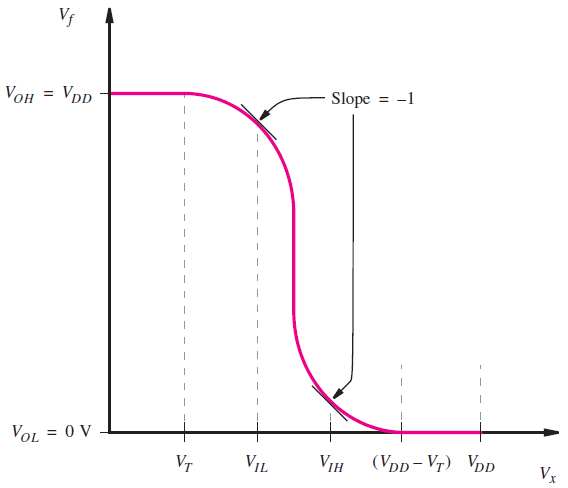
\includegraphics[scale=0.45]{../EJ1/Recursos/logic_leves.PNG} &
        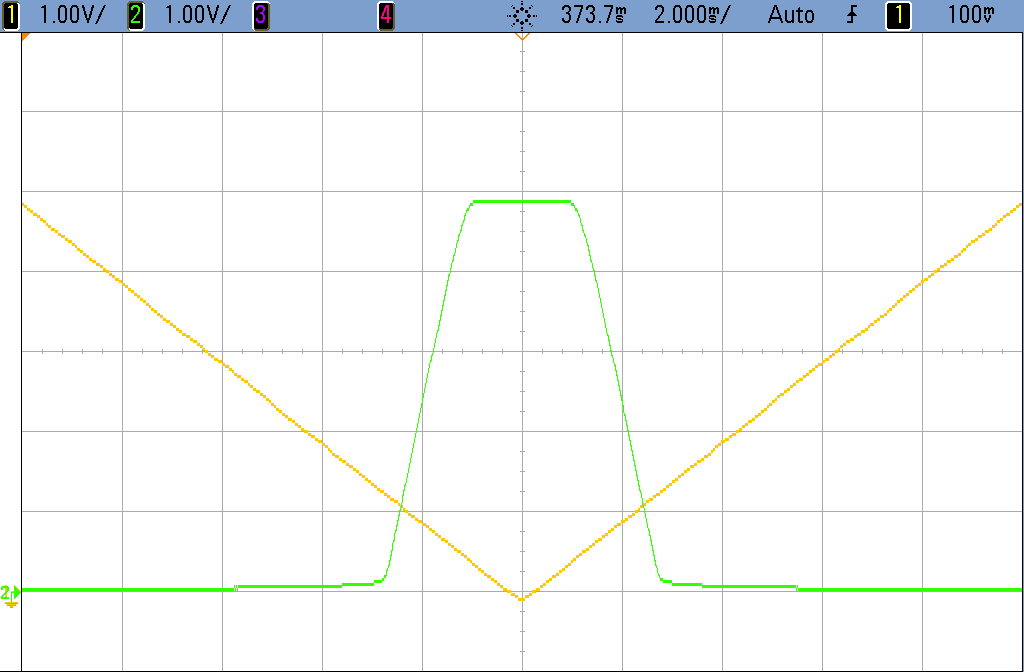
\includegraphics[scale=0.23]{../EJ1/Mediciones/Osciloscopio/Segundo_Intento/Voltage_Levels_RTL/cropped_scope_3.png}
    \end{tabular}
    \caption{$V_o(V_i)$ y medici\'on entrada(amarilla) y salida(verde).}
    \label{fig:logic_levels}
\end{figure}

\begin{table}[H]
    \centering
    \begin{tabular}{c c c c c c c}
        Circuito & VIH & VIL & VOH & VOL & NMH & NML \\
        \hline \\
        RTL & $1.33V$ & $0.28V$ & $4.89V$ & $0.11V$ & $3.55V$ & $0.16V$ \\
        TTL & $0.56V$ & $0.3V$ & $4.89V$ & $0.01V$ & $4.32V$ & $0.29V$ \\
        MOS & $2.7V$ & $1.94V$ & $4.89V$ & $0.04V$ & $2.19V$ & $1.89V$ \\
        CMOS & $1.7V$ & $2.89V$ & $4.94V$ & $0.04V$ & $3.23V$ & $2.85V$ \\
        \hline
    \end{tabular} 
    \caption{Resultados de los niveles de tensi\'on}
\end{table}

\begin{table}[H]
    \centering
    \begin{tabular}{c c c c c c c}
        Circuito & VIH & VIL & VOH & VOL & NMH & NML \\
        \hline \\
        RTL & $1.31V$ & $0.25V$ & $4.89V$ & $0.13V$ & $3.58V$ & $0.12V$ \\
        TTL & $0.55V$ & $0.31V$ & $4.89V$ & $0.01V$ & $4.33V$ & $0.29V$ \\
        MOS & $2.53V$ & $2.1V$ & $4.88V$ & $0.01V$ & $2.34V$ & $2.09V$ \\
        CMOS & $1.44V$ & $2.83V$ & $4.94V$ & $0.04V$ & $3.49V$ & $2.79V$ \\
        \hline
    \end{tabular} 
    \caption{Resultados de los niveles de tensi\'on con carga de $C = 1nF$}
    \label{table:voltage_levels_charged}
\end{table}

\subsubsection{An\'alisis de resultados}
En primer lugar, de RTL a TTL disminuye el valor de VIH de forma esperado, ya que con la etapa de entrada con el primer transistor, se necesita menos tensi\'on
con la cual polarizarlo y eventualmente saturar el transistor de salida. Por otro lado, es de esperar que los valores de VOH entre tales tecnolog\'ias no difieran,
dado que al corte se comporta de igual manera en la malla de salida, no obstante se asume que la diferencia entre valores de VOL es causada por el incremento en la condici\'on
de saturaci\'on en el caso de TTL, puesto que al estar elevando la corriente de colector el punto de polarizaci\'on se desplaza a una menor tensi\'on.

En segundo lugar, es de esperar que entre las topolog\'ias usadas como MOS y CMOS, los valores de VOL no difieran, ya que est\'a impuesto por la red pull-down realizada con un transistor NMOS,
mientras que la diferencia de uno a otro es el pull-up, lo cual puede denotarse en el incremento de VOH para CMOS.

En t\'erminos generales, puede observarse que los niveles de salida mas fuertes son entregados por el caso CMOS, con un m\'argen de ruido para ambos casos mayor en cuanto a la distribuci\'on.


Desde otro punto de vista, en la Tabla. \ref{table:voltage_levels_charged} se puede observar que en el resultado de las mediciones habiendo cargado las compuertas, es notable destacar que la que mayor mantiene sus valores
es la compuerta CMOS.

\subsection{Tiempos de operaci\'on}
De la expresi\'on l\'ogica ideal a la implementaci\'on en dispositivos f\'isicos existen limitaciones que acarrean inconvenientes y pueden provocar que el comportamiento
resultante no sea el esperado, entre estas caracter\'isticas se encuentran los tiempos de transici\'on que describen el retardo del dispositivo en pasar una salida del estado bajo al alto y viceversa, as\'i como tambi\'en los tiempos
de propagaci\'on que requiere el dispositivo para reflejar los cambios de la entrada en la salida.

\subsubsection{Proceso de medici\'on}
Empleando un generador de funciones se configura una se\~nal cuadrada con duty $50\%$ con un valor de tensi\'on $5 V_{PP}$ y una tensi\'on de offset $2.5V$, luego utilizando un osciloscopio se mide con dos canales
la se\~nal de entrada y de salida, configurando el trigger para dos escenarios alternativos de rise y fall, de esta forma se logra capturar ambos escenarios de inversi\'on ya sea de estado alto a bajo como de bajo a alto. La frecuencia debe ser baja al igual que antes,
seg\'un convenga inferior a $f = 100Hz$.
Finalmente, se descargan los datos de entrada y salida en archivos .csv para ser procesados por un software. Se determina el tiempo de transici\'on de la salida entre el $10\%$ y el $90\%$, mientras que el tiempo de propagaci\'on se da entre la entrada y salida al $50\%$.

\begin{figure}[H]
    \centering
        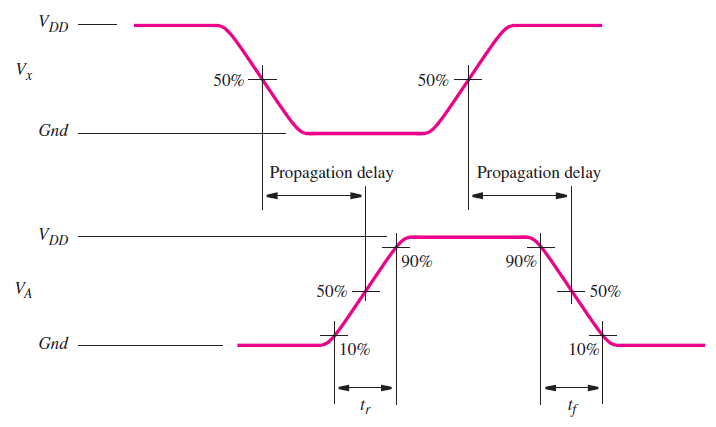
\includegraphics[scale=0.6]{../EJ1/Recursos/time_logic.PNG}
    \caption{Definici\'on te\'orica de los tiempos a medir}
    \label{fig:time_logic}
\end{figure}

\begin{figure}[H]
    \centering
        \begin{tabular}{c c}
            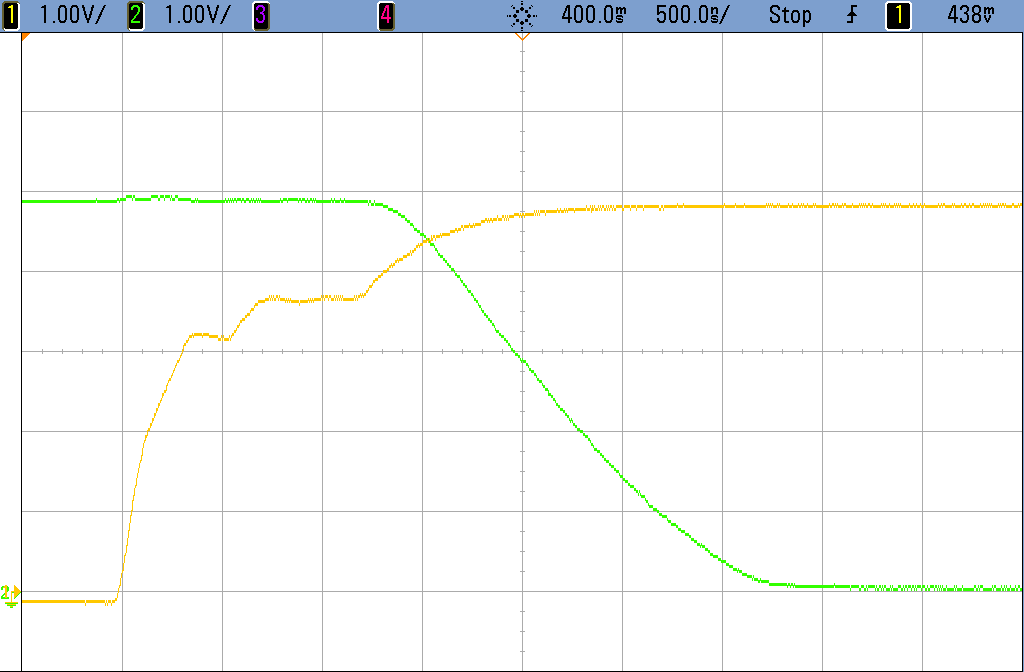
\includegraphics[scale=0.20]{../EJ1/Mediciones/Osciloscopio/Segundo_Intento/Times_RTL/cropped_scope_37.png} &
            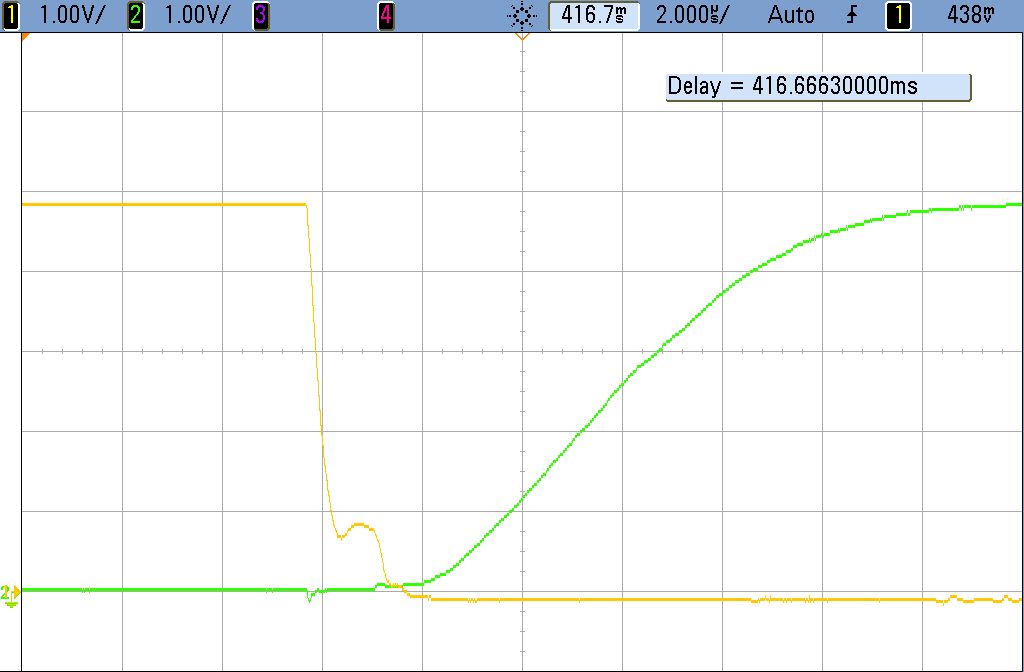
\includegraphics[scale=0.20]{../EJ1/Mediciones/Osciloscopio/Segundo_Intento/Times_RTL/cropped_scope_39.png}
        \end{tabular}
    \caption{Casos ejemplo de medici\'on de los tiempos}
    \label{fig:operation_times}
\end{figure}

\begin{table}[H]
    \centering
    \begin{tabular}{c c c c c}
        Circuito & Prop. de alto a bajo & Prop. de bajo a alto & Trans. de alto a bajo & Trans. de bajo a alto \\
        \hline \\
        RTL & $5.49\mu s$ & $1.88\mu s$ & $1.37\mu s$ & $6.12\mu s$ \\
        TTL & $2.81\mu s$ & $55ns$ & $57.2ns$ & $57n s$ \\
        MOS & $15.3\mu s$ & $185ns$ & $177ns$ & $27.4\mu s$ \\
        CMOS & $710ns$ & $720ns$ & $412ns$ & $504ns$ \\
        \hline
    \end{tabular}
    \caption{Medici\'on de los tiempos de operaci\'on sin carga}
\end{table}

\begin{table}[H]
    \centering
    \begin{tabular}{c c c c c}
        Circuito & Prop. de alto a bajo & Prop. de bajo a alto & Trans. de alto a bajo & Trans. de bajo a alto \\
        \hline \\
        RTL & $11.2\mu s$ & $2.75\mu s$ & $2.8\mu s$ & $29.2\mu s$ \\
        TTL & $9.68\mu s$ & $72ns$ & $206ns$ & $27.8 \mu s$ \\
        MOS & $23.4\mu s$ & $210ns$ & $182ns$ & $51.2\mu s$ \\
        CMOS & $750ns$ & $745ns$ & $434ns$ & $532ns$ \\
        \hline
    \end{tabular}
    \caption{Medici\'on de los tiempos de operaci\'on con $C = 1nF$}
\end{table}

\subsubsection{An\'alisis de resultados}
Las cargas capacitivas agregadas a las salidas de las compuertas produce un incremento en los tiempos de operaci\'on medidos, pero adem\'as,
resulta de inter\'es comparar las diferencias entre las tecnolog\'ias.
En primer lugar, entre las tecnolog\'ias RTL y TTL, se puede observar una amplia diferencia que es esperada, dado que el mismo transistor empleando en RTL,
tiene una etapa previa implementada justamente para reducir los tiempos de operaci\'on utilizando m\'as corrientes para controlar los procesos de apagado y encendido de las junturas.

Por otro lado, al momento de cargar con una determinada capacidad las compuertas, la que menos variaci\'on presenta es la CMOS.

\subsection{Corrientes m\'aximas}
La interconexi\'on de un conjunto amplio de compuertas l\'ogicas puede requerir un gran consumo de corriente para las salidas de las mismas, con lo cual es necesario
determinar las m\'aximas corrientes de estado alto y estado bajo que puede soportar los circuitos empleados, puesto que de esta forma puede estimarse el m\'aximo n\'umero de compuertas a conectar.

\subsubsection{Proceso de medici\'on}
Como se puede observar en la Fig. \ref{fig:maximum_current_process} el proceso de medici\'on consiste en, para cada estado, utilizar una carga en la salida
variable con el objetivo de ir variando el valor y observando cu\'al es la tensi\'on a la salida. Para cada caso, se considera que la corriente m\'axima es aquella para la cual
en la salida se observa el nivel de tensi\'on que define el l\'imite del estado de la salida, sea VOH o VOL.

\begin{figure}[H]
    \centering
        \begin{tabular}{c c}
            \includegraphics[scale=0.45]{../EJ1/Recursos/maximum_current.png} &
            \includegraphics[scale=0.45]{../EJ1/Recursos/maximum_current_low.png} 
        \end{tabular}
    \caption{Proceso de medici\'on de m\'axima corriente}
    \label{fig:maximum_current_process}
\end{figure}

\begin{table}[H]
    \centering
    \begin{tabular}{c c c}
        Circuito & IOH & IOL \\
        \hline \\
        RTL & $14.4 \mu A$ & $488\mu A$ \\
        TTL & $14.6 \mu A$ & $13.1 \mu A$ \\
        MOS & $11.5 \mu A$ & $249 \mu A$ \\
        CMOS & $15.2mA$ & $135\mu A$ \\
        \hline
    \end{tabular}
    \caption{Mediciones de corriente m\'axima sin carga}
\end{table}

\begin{table}[H]
    \centering
    \begin{tabular}{c c c}
        Circuito & IOH & IOL \\
        \hline \\
        RTL & $11.1 \mu A$ & $1.13m A$ \\
        TTL & $10.2 \mu A$ & $49.5 \mu A$ \\
        MOS & $12.4 \mu A$ & $37.7 \mu A$ \\
        CMOS & $21.3mA$ & $102\mu A$ \\
        \hline
    \end{tabular}
    \caption{Mediciones de corriente m\'axima con carga $C = 1nF$}
\end{table}

\subsubsection{An\'alisis de resultados}
Las implementaciones realizadas RTL, TTL, MOS tienen una corriente similar de IOH, lo cual tiene sentido ya que tal es provista
por la resistencia de pull-up que cada caso es similar, aproximadamente en $R = 10k \Omega$ con la distinci\'on real provocada por la tolerancia y el comportamiento
de la malla de salida de los dispositivos. Pero en definitiva los valores son cercanos por esta raz\'on.

A pesar de esto \'ultimo, cada una de tales tecnolog\'ias difiere de las dem\'as en la corriente IOL justamente porque est\'a definida por el control de la condici\'on de saturaci\'on en los BJT, y la zona \'ohmica en el caso
de los MOSFET. No obstante, dado que en el circuito CMOS los MOSFETS son complementarios, no se encontr\'o razonamiento por el cual la corriente IOH sea tan diferente con respecto de IOL, se asume que es por las condiciones
en las que pudieran encontrarse los modelos usados.

\subsection{Conclusiones}
